%\chapter{3D-Stereokalibrierung und Szenenrekonstruktion mit reellen Daten und Kameras unterschiedlicher Auflösung}
\label{sec:realAuf} 

\section{Ergebnisse einer Stereoanalyse mit Kameras unterschiedlicher Auflösung}

Für den Test, ob die Szenerekonstruktion im Realbeispiel auch mit unterschiedlichen Kameraauflösungen funktioniert, wird die Kameramatrix $K'$ von $C'$ künstlich skaliert. Wie aus Kapitel \ref{sec:CameraModels}, hat diese die Form

%mn Kapitel \nameref{sec:basisTransformation} wurden die einzelnen Bauteile der Kameramatrix genau beschrieben. Die Kameramatrix $K'$ aus Matlab für die Canon 60D gegeben.


\begin{gather}
K'_{[1:1]}=\begin{bmatrix}
k_x\zeta&s&V_{\sigma,x}\\
0&k_y\zeta&V_{\sigma,y}\\
0&0&1
\end{bmatrix}
\end{gather} \\
.

%$\alpha_x$ und $\alpha_y$ setzen sich auch dem Abstand des Kamerazentrums zum Hauptpunkt zusammen, welcher in dieser Arbeit als mit $\zeta$ bezeichnet wurde, und den Kantenlängen der Pixel auf dem Sensor $m_x$ und $m_y$. 

Um die Auflösung von $K'$ zu verändern, werden die Matrixeinträge $k_x \zeta$ und $k_y \zeta$ jeweils noch um eine beliebige Skalierung erweitert. Für den Test wird $K'$ drei mal unterschiedlich skaliert und zwar mit den Verhältnissen $[5:2],\, [1:2]$ und $[1.2:2.3]$.  

%wird auf $\alpha_x$ und $\alpha_y$ jeweils ein beliebiger Faktor dazu multipliziert. Zum Beweis, dass die Rekonstruktion der externen Kameraparameter und die Szenerekonstruktion, bei egal welcher Skalierung, die ähnlichen Ergebnisse liefern, wurde die Kameramatrix $K'$ mit den Verhältnissen $[2:2], \, [5:2],\, [2:1], \, [1:2]$ und $[1.2:2.3]$ skaliert. 

\begin{gather*}
%K'_{[2:2]}=	
%\begin{bmatrix}
%k_x\zeta \cdot 2 &s&V_{\sigma,x} \cdot 2\\
%0&k_y\zeta \cdot 2&V_{\sigma,y} \cdot 2\\
%0&0&1
%\end{bmatrix}\\
K'_{[5:2]}=	
\begin{bmatrix}
k_x\zeta \cdot 5 &s&V_{\sigma,x} \cdot 5\\
0&k_y\zeta \cdot 2&V_{\sigma,y} \cdot 2\\
0&0&1
\end{bmatrix}\\
%K'_{[2:1]}=	
%\begin{bmatrix}
%k_x\zeta \cdot 2 &s&V_{\sigma,x} \cdot 2\\
%0&k_y\zeta \cdot 1&V_{\sigma,y} \cdot 1\\
%0&0&1
%\end{bmatrix}\\
K'_{[1:2]}=	
\begin{bmatrix}
k_x\zeta \cdot 1 &s&V_{\sigma,x} \cdot 1\\
0&k_y\zeta\cdot 2&V_{\sigma,y} \cdot 2\\
0&0&1
\end{bmatrix}\\
K'_{[1.2:2.3]}=	
\begin{bmatrix}
k_x\zeta \cdot 1.2 &s&V_{\sigma,x} \cdot 1.2\\
0&k_y\zeta \cdot 2.3&V_{\sigma,y} \cdot 2.3\\
0&0&1
\end{bmatrix}\\
\end{gather*}


%Die Formulierung, dass die jeweils neu rekonstruierten Szenen ähnlich sind, wurde deshalb verwendet, da durch die zuvorigen Fehler der korrespondierenden Punkte und später, bei der Triangulierung, durch die \textit{Sampson-Approximation} Abweichungen auftreten können. 
Von den detektierten korrespondierenden Bildpunkten des SURF-Algorithmus werden die Bildpunkte des zweiten Bildes von $C'$ auch um die selben Verhältnisse skaliert.

\begin{gather}
%	m_{\sigma[2:2]}=
%	m_\sigma \cdot
%	\begin{pmatrix}
%2&0&0\\
%0&2&0\\
%0&0&1	
%	\end{pmatrix}\\
	m_{\sigma[5:2]}=
m_\sigma \cdot
\begin{pmatrix}
	5&0&0\\
	0&2&0\\
	0&0&1	
\end{pmatrix}\\
	m_{\sigma[1:2]}=
m_\sigma \cdot
\begin{pmatrix}
	1&0&0\\
	0&2&0\\
	0&0&1	
\end{pmatrix}\\
	m_{\sigma[1.2:2.3]}=
m_\sigma \cdot
\begin{pmatrix}
	1.2&0&0\\
	0&2.3&0\\
	0&0&1	
\end{pmatrix}
\end{gather}


Der Szenenrekonstruktionsalgorithmus wird für jede Kameraauflösung getestet. Die Abbildungen \ref{fig:RecT52}, \ref{fig:RecT52} und \ref{fig:RecT1223} zeigen jeweils die vier Lösungen für $T'$, welche sich bei der Bestimmung der extrinsischen Parameter bei unterschiedlichen Kameraauflösungen ergaben. Zu beobachten ist, dass sich die Lösungen bei unterschiedlichen Auflösungen nicht unterscheiden. Die geringen Abweichungen in den Nachkommastellen sind auf die Ungenauigkeiten der Bilddaten zurückzuführen. Durch die Skalierung der Bildkoordinaten in die neuen Sensorkoordinatensysteme werden auch deren Abweichungen mit skaliert. 

%Mit den veränderten Bildpunkten und Kamermatrix $K'$ wurde 
%
%
%Als Beweise werden im folgenden vier Beispiele für die vier Lösungen der rekonstruierten Translationsmatrizen $R'$ aufgezeigt. Des Weiteren werden die 3D-Plots und 2D-Plots der rekonstruierten Szenen bei unterschiedlich Auflösungen im Vergleich mit der Szene bei gleichen Auflösungen gezeigt. Die Koordinaten sind in unskalierten Pixeleinheiten gegeben. Die Originalszene ist in Abbildung 7.15 und 7.16 zu sehen. Zu beachten ist, das die Ausgabe des 3D Plots in \textit{Mathematica} manchmal rechtsdrehend, manchmal linksdrehend dargestellt sind, weshalb der Eindruck aufkommt, die Szene und die Kameraposition seien gespiegelt dargestellt. Dies leider auf ein generellen Darstellungsproblem von 3D-Plots in Mathematica zurückzuführen. Dieses kann mit zusätzlichem Code bereinigt werden, wurde aber zu diesem Zeitpunkt noch nicht implementiert. 




\begin{figure}[!htb]
	\minipage{0.48\textwidth}
	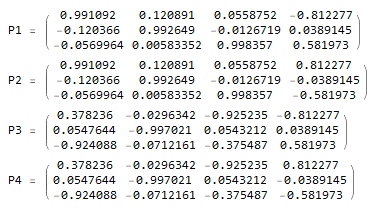
\includegraphics[width=\linewidth]{images/R_11.png}
	\caption[Vier Lösungen für $T$ bei gleicher Kameraauflösung]{Zeigt die Die rekonstruierte Matrix $T'$ bei unveränderter Auflösung. Die Auflösungen von $C_\delta$ und $C'_\delta$ sind die selben.}
	\label{fig:T11}
	\endminipage\hfill
	\minipage{0.48\textwidth}
	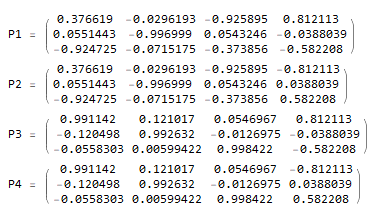
\includegraphics[width=\linewidth]{images/R_52.png}
	\caption[Vier Lösungen für $T$ bei $K'$ mit 5:2]{Zeigt die rekonstruierte Matrix $T'$ wenn $K'$ mit einem Verhältnis von $[5:2]$ skaliert wurde}
	\label{fig:T52}
	\endminipage\hfill
\end{figure}
\begin{figure}[!htb]
	\minipage{0.48\textwidth}
	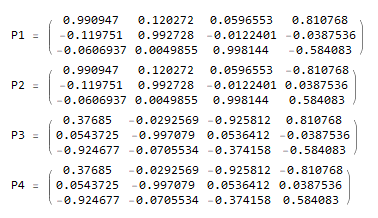
\includegraphics[width=\linewidth]{images/R_12.png}
	\caption[Vier Lösungen für $T$ bei $K'$ mit 1:2]{Zeigt die rekonstruierte Matrix $T'$ wenn $K'$ mit einem Verhältnis von $[1:2]$ skaliert wurde}
	\label{fig:T12}
	\endminipage\hfill
	\minipage{0.48\textwidth}
	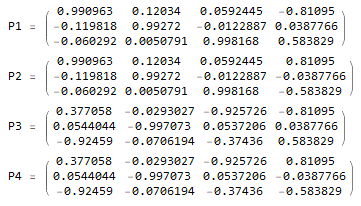
\includegraphics[width=\linewidth]{images/R_12_23.png}
	\caption[Vier Lösungen für $T$ bei $K'$ mit 1.2 : 2.3]{Zeigt die rekonstruierte Matrix $T'$ wenn $K'$ mit einem Verhältnis von $[1.2:2.3]$ skaliert wurde}
	\label{fig:T1223}
	\endminipage\hfill
\end{figure}
\pagebreak

Die Abbildungen \ref{fig:RecT52}, \ref{fig:RecT12} und \ref{fig:RecT1223} zeigen einmal die Rekonstruierten Punkte in einem 3D-Plot und daneben den 2D-Plot. Auch hier kann beobachtet werden, dass es immer zu den gleichen rekonstruierten Szenen kommt. In Abbildung \ref{fig:RecT12} ist die Rekonstruktion in einem links drehendem Koordinatensystem geplottet, weshalb die Rekonstitution spiegelverkehrt wirkt. 

%\begin{figure}[!htb]
%	\centering
%	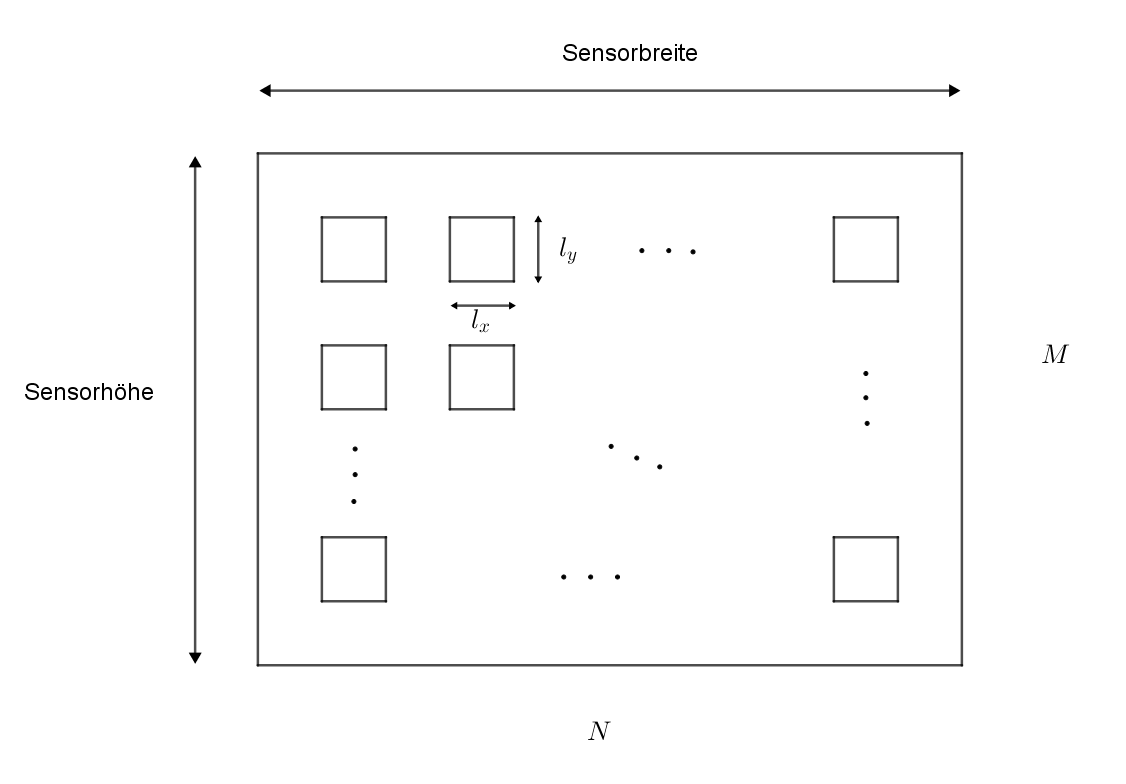
\includegraphics[width=.7\linewidth]{images/Bildsensor_mit_Pixel.png}
%	\caption[Aufbau CMOS Sensor]{Rechteckiger Bildsensor mit darauf sich befindendenden quadratischen Sensorelementen. Vergleiche \cite{Photonik}} 
%	\label{fig:Sensor}
%\end{figure}

\begin{figure}[!htb]
	\minipage{0.48\textwidth}
	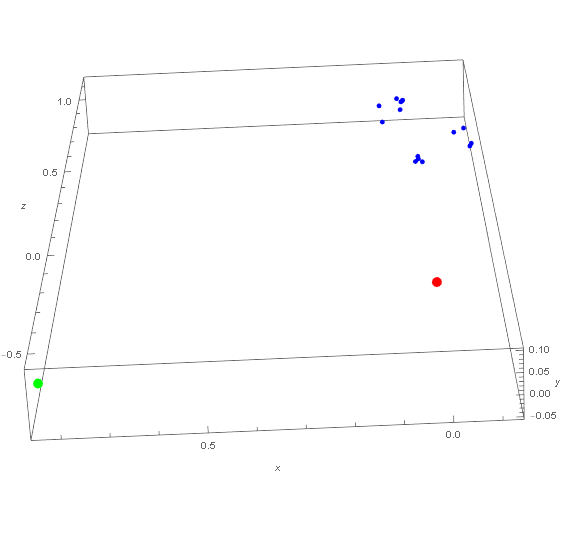
\includegraphics[width=\linewidth]{images/Reconstrution3D_52.png}
%	\caption{$C$ und $C'$ haben die selbe Auflösung eingestellt}
	\endminipage\hfill
	\minipage{0.48\textwidth}
	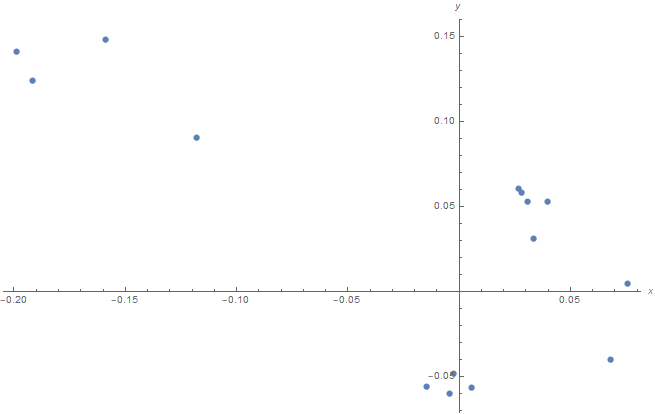
\includegraphics[width=\linewidth]{images/Reconstrution2D_52.png}
%	\caption{$C$ und $C'$ haben unterschiedliche Auflösungen eingestellt}
	\endminipage\hfill
	\caption[Rekonstruierte Szene bei $K'$ = 5:2]{Rekonstruierte Szene, wenn $K'$ mit einem Verhältnis von $[5:2]$ skaliert wurde}
	\label{fig:RecT52}
\end{figure}
\begin{figure}[!htb]
	\minipage{0.48\textwidth}
	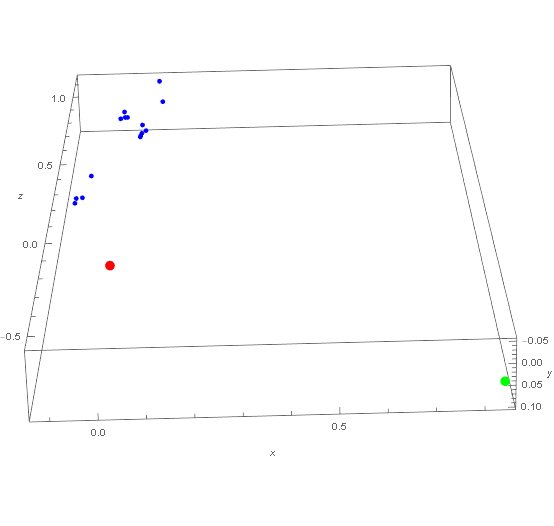
\includegraphics[width=\linewidth]{images/Reconstrution3D_12.png}
	%	\caption{$C$ und $C'$ haben die selbe Auflösung eingestellt}
	\label{fig:awesome_image1}
	\endminipage\hfill
	\minipage{0.48\textwidth}
	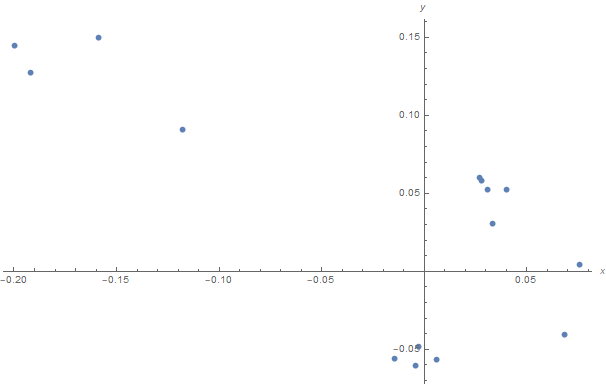
\includegraphics[width=\linewidth]{images/Reconstrution2D_12.png}
	%	\caption{$C$ und $C'$ haben unterschiedliche Auflösungen eingestellt}
	\label{fig:awesome_image2}
	\endminipage\hfill
	\caption[Rekonstruierte Szene bei $K'$ = 1:2]{Rekonstruierte Szene, wenn $K'$ mit einem Verhältnis von $[1:2]$ skaliert wurde}
	\label{fig:RecT12}
\end{figure}
\begin{figure}[!htb]
	\minipage{0.48\textwidth}
	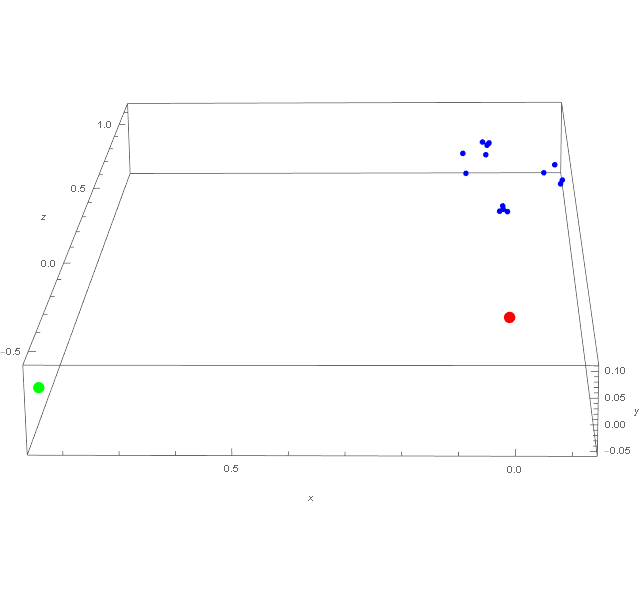
\includegraphics[width=\linewidth]{images/Reconstrution3D_12_23.png}
	%	\caption{$C$ und $C'$ haben die selbe Auflösung eingestellt}
	\label{fig:awesome_image1}
	\endminipage\hfill
	\minipage{0.48\textwidth}
	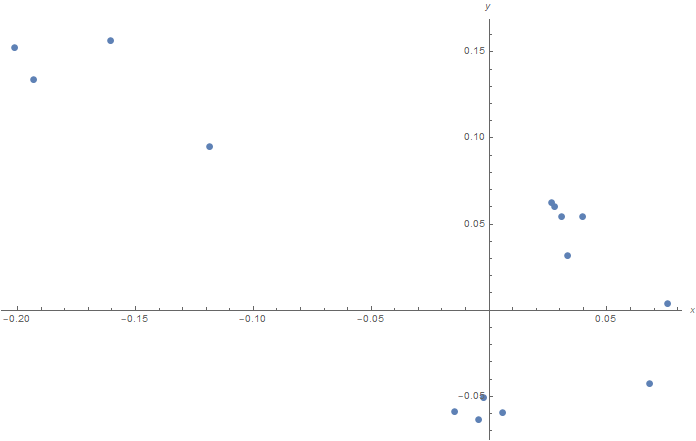
\includegraphics[width=\linewidth]{images/Reconstrution2D_12_23.png}
	%	\caption{$C$ und $C'$ haben unterschiedliche Auflösungen eingestellt}
	\label{fig:awesome_image2}
	\endminipage\hfill
	\caption[Rekonstruierte Szene bei $K'$ = 1.2:2.3]{Rekonstruierte Szene, wenn $K'$ mit einem Verhältnis von $[1.2:2.3]$ skaliert wurde}
	\label{fig:RecT1223}
\end{figure}

